% Created 2020-08-20 Thu 18:54
% Intended LaTeX compiler: pdflatex
\documentclass[a4paper, jou, 11pt]{apa6}
 \usepackage[nodoi]{apacite}
 \usepackage[british, english]{babel}
 \usepackage{inputenc}
 \usepackage{amsmath}
 \usepackage{graphicx}
 \usepackage{csquotes}
 \usepackage[hyphens]{url}
 \usepackage[T1]{fontenc}
 \usepackage{lmodern}
 \usepackage{hyperref}
\usepackage[utf8]{inputenc}
\usepackage[T1]{fontenc}
\usepackage{graphicx}
\usepackage{grffile}
\usepackage{longtable}
\usepackage{wrapfig}
\usepackage{rotating}
\usepackage[normalem]{ulem}
\usepackage{amsmath}
\usepackage{textcomp}
\usepackage{amssymb}
\usepackage{capt-of}
\usepackage{hyperref}
\shorttitle{Differences in Body Image}
\journal{horizonofreason.com}
\ccoppy{\ccLogo \enspace Creative Commons Attribution-ShareAlike 3.0}
\affiliation{Monash University}
\abstract{Abstract: This study measures the current and ideal body shape of the subject and the body shape of the most attractive other sex. The results confirm previous research which found that body dissatisfaction for females is significantly higher than for men. The research also found a mild positive correlation between age and ideal body shape for women and between age and the female body shape found most attractive by men.}
\keywords{psychology, body image, physical attraction}
\rightheader{Third Hemisphere Publishing}
\authornote{This paper was prepared for the \emph{Psychology 1A} course of Monash University, Melbourne.}
\author{Peter Prevos}
\date{\today}
\title{Experimental Verification of Differences in Body Image Between Men and Women}
\hypersetup{
 pdfauthor={Peter Prevos},
 pdftitle={Experimental Verification of Differences in Body Image Between Men and Women},
 pdfkeywords={},
 pdfsubject={},
 pdfcreator={Emacs 26.3 (Org mode 9.3.7)}, 
 pdflang={English}}
\begin{document}

\maketitle
1\#+LATEX\textsubscript{HEADER}: \note{20 February 2005}

\section{Introduction}
\label{sec:org04a3de9}
The most important indication of beauty for women in Western societies is the prevailing ideal of thinness. This ideal causes many women to desire an unrealistically thin body image \cite{lamb_body_1993}. The preoccupation with thinness is a recent cultural development as the perception of female body shapes has changed significantly over the past decades. In the early 1940's it was found that others perceived people with thin ectomorph bodies as nervous, submissive and socially withdrawn. By the late 1980's this perception had changed, and thin people were considered to be the most sexually appealing \cite{turner_influence_1997}.

Several researchers have found that the female body depicted in the media has become increasingly thin. Using \emph{Playboy} models as a proxy for what is perceived as beautiful, bust and hip measurements of centrefold models show that between 1960 and 1979 there was a trend towards non-curvaceousness of women. This trend was, however, reversed in the early 1990s, as visualised in Figure \ref{playboy} \cite{garner_cultural_1980,turner_influence_1997,sypeck_cultural_2006,wiseman_cultural_1992}.

\begin{figure}[htbp]
\centering
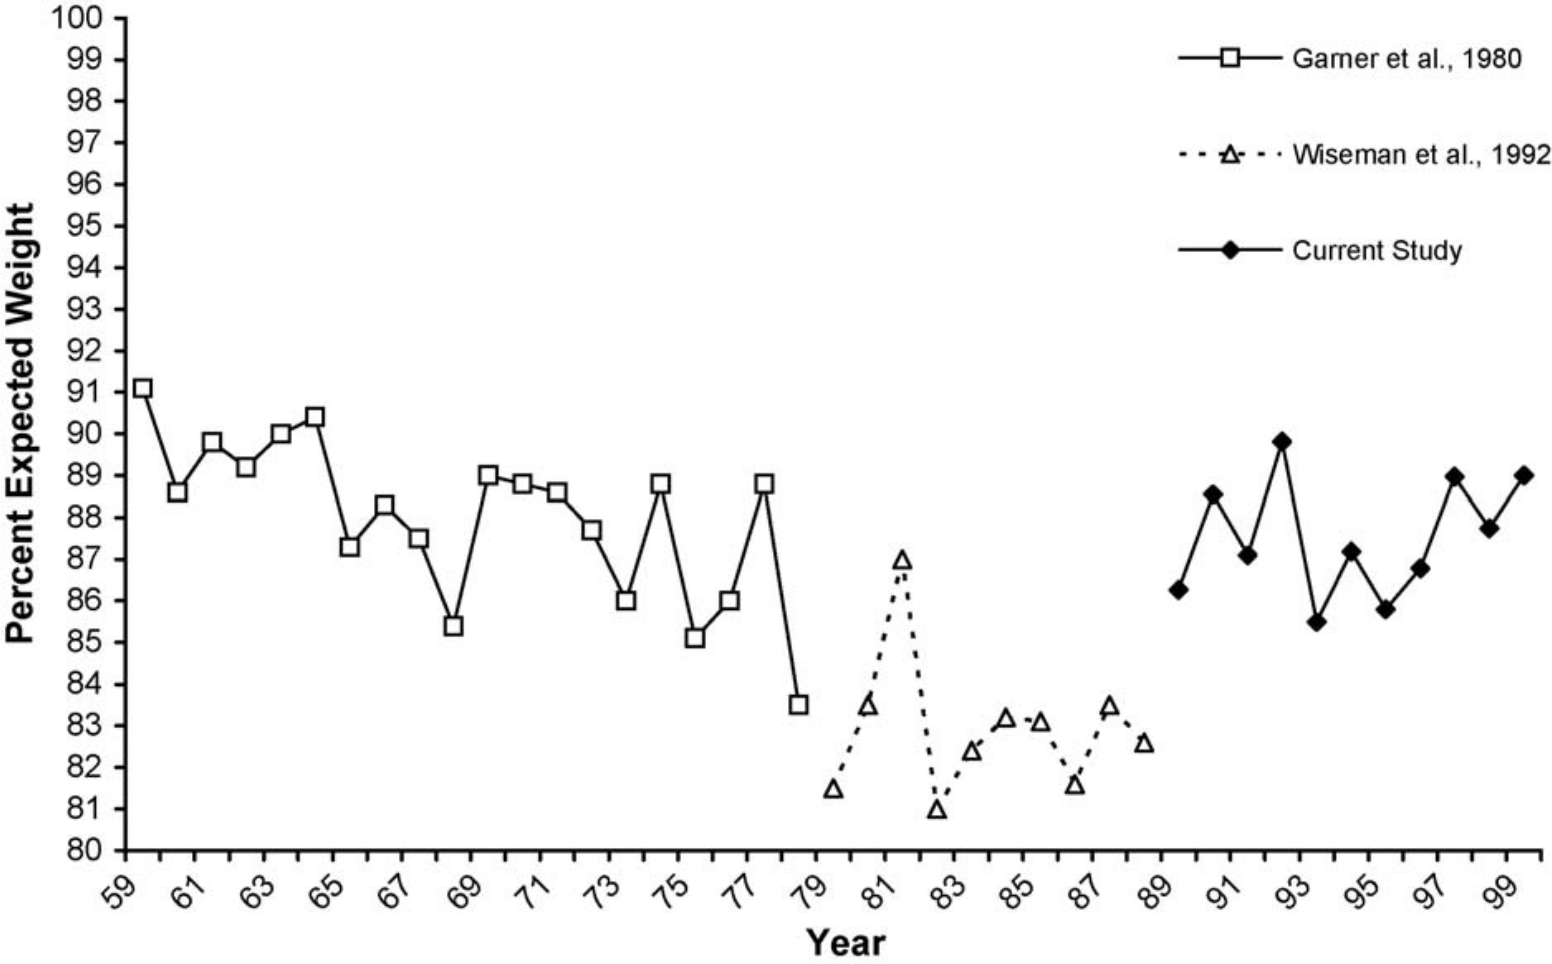
\includegraphics[width=.9\linewidth]{playboy.png}
\caption{Percent normative weight of the Playmates as a function of time (Sypeck et al., 2006). \label{playboy}}
\end{figure}

Parallel to the decrease in size of the ideal body shape for women, the dissatisfaction that women have with their body shape increased \cite{cash_how_2004}. In recent years, females were found to be more likely to judge themselves overweight than males. This tendency was strongest in adolescent and young adult women \cite{fallon_sex_1985,tiggeman_development_1990,tiggeman_body-size_1992}. Concerns with body image have been linked to a decrease in self-esteem and an increase in dieting among young women \cite{hill_eating_1992}. An increase in dieting among young women has been identified as an indicator of the onset of eating disorders such as \emph{anorexia nervosa} and \emph{bulimia nervosa} \cite{barker_body_2003,fear_prevalence_1996,lamb_body_1993}.

Numerous studies have been undertaken to study body dissatisfaction in recent years \cite{fallon_sex_1985,tiggeman_development_1990,tiggeman_body-size_1992,lamb_body_1993,abel_relationship_1996,byrne_should_1996,fear_prevalence_1996,cash_how_2004}. They generally concluded that approximately one-third of men and almost three quarter of women rate their current figure as larger than ideal and that body dissatisfaction among women is much larger than for men. \citeA{fallon_sex_1985} also found that men judge the female figure they found most attractive as heavier than women's ratings of the ideal body shape.
\subsection{Hypotheses}
\label{sec:org22c6220}
The first hypothesis tested in this study is that the ideal body shape for women (\(ideal\)) is thinner than their current self-assessed body image (\(current\)) and the ideal body shape for men is heavier than their current body shape.

$$H_{1w}: ideal - current < 0 $$

$$H_{1m}: ideal - current > 0 $$

Some research has also been undertaken to determine generational differences in body shape preferences \cite{lamb_body_1993}. \citeA{tiggeman_development_1990} researched body size dissatisfaction for children, adolescents and adults and found significant differences between the age groups. It should be noted that they used different types of body image scales for each age group. \citeA{lamb_body_1993} compared two generations and found significance gender and cohort differences. These cohort differences confirm the recent increase in body dissatisfaction and eating disorders among mainly young women. In this study, the ideal image for females of different ages and the most attractive female body shape, as judged by men, will be determined for various age groups. The second hypothesis of this study is that there is a positive correlation between age and the ideal figure for females and between age and the female body image that men find most attractive.

$$H_2: R_{ideal,age} >0$$
\section{Method}
\label{sec:orgc4045cc}
\subsection{Participants}
\label{sec:org4f8bb45}
The participants of the survey are unsolicited visitors to the Monash University website. Most participants were students undertaking the psychology course. No socioeconomic information is available. The survey data contains 166 surveys completed between 3 January 2003 and 6 March 2004, of which 59 male and 107 female. Fourteen surveys were only partially completed and were not considered in the analysis. Table \ref{gender-age} shows the age distribution over the full data set. The cohorts taken into account for this survey are men and women between 16 and 30 years of age. 

% latex table generated in R 4.0.2 by xtable 1.8-4 package
% Thu Aug 20 18:54:17 2020
\begin{table}[ht]
\centering
\begin{tabular}{rrrrrr}
  \hline
 & $<$ 16 & 16--30 & 31--50 & $>$ 50 & Sum \\ 
  \hline
Female & 1 & 56 & 46 & 4 & 107 \\ 
  Male & 0 & 29 & 24 & 6 & 59 \\ 
  Sum & 1 & 85 & 70 & 10 & 166 \\ 
   \hline
\end{tabular}
\caption{Age profile of survey participants} 
\label{gender-age}
\end{table}

\subsection{Materials}
\label{sec:org3899456}
The questionnaire consisted of seven questions regarding body shape and a further five questions regarding age, gender and possible concerns regarding body shape and dieting. Question 1 (current body shape), 2 (ideal body shape) and question 6 (body shape of the other gender found most attractive) and the questions about gender and age of the on-line questionnaire were used for analysis. The remaining survey results have not been considered.

Participants were asked to compare a set of nine drawings, showing an increasing body size (Figure \ref{scale}). Subjects were invited to score the first seven questions between one and nine. This type of survey has been widely used in similar research regarding body dissatisfaction \cite{abel_relationship_1996,byrne_should_1996,fallon_sex_1985,fear_prevalence_1996,hill_eating_1992,lamb_body_1993,tiggeman_development_1990,tiggeman_body-size_1992}. 

\begin{figure}[htbp]
\centering
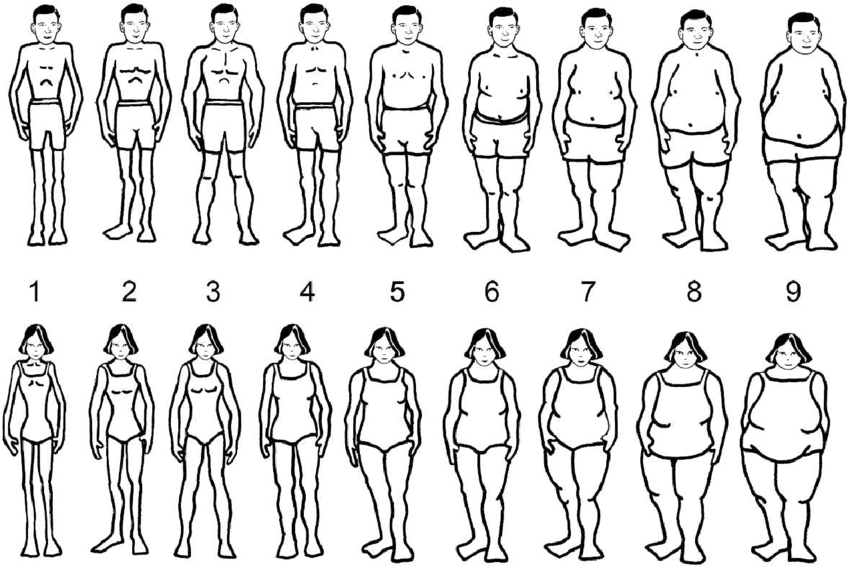
\includegraphics[width=.9\linewidth]{BodyScale.png}
\caption{Body shape measurement scale. \label{scale}}
\end{figure}

The independent variables for this experiment are the gender and age of the participants. The dependent variables under consideration are the perceived current body shape (\(current\)), the ideal body shape (\(ideal\)) and the body shape of the other gender found most attractive (\(other\)). 

Of the 16--30 cohort, 29 results were submitted by men and 29 by women. A random sample of 29 of the results provided by women and all responses submitted by men in this cohort were considered to ensure symmetry in the data. The complete data set was used to determine the correlations between age and ideal female figures for both men and women.
\section{Results}
\label{sec:org88731a3}
\subsection{Body Image}
\label{sec:org5a55694}
The arithmetic mean and standard deviation of the three questions under consideration are summarised in Table \ref{results}. The results have not been tested for statistical significance. The results show that for women, the average current figure is larger than the average ideal, while for men the perceived current body shape is much closer to the ideal. The percentage of women that considered their current body shape larger than the ideal (\(current-ideal>0\)) is 75.9, while only 37.9 of men thought that their current body shape was larger than their ideal.

% latex table generated in R 4.0.2 by xtable 1.8-4 package
% Thu Aug 20 18:54:18 2020
\begin{table}[ht]
\centering
\begin{tabular}{rrlll}
  \hline
 & $n$ & $Current$ & $Ideal$ & $Current-Ideal$ \\ 
  \hline
F &  29 & 3.93(1.19) & 3.03(0.94) & 0.9(0.86) \\ 
  M &  29 & 4.14(1.55) & 4.03(0.73) & 0.1(1.37) \\ 
   \hline
\end{tabular}
\caption{Mean and standard deviation of body image} 
\label{results}
\end{table}

\subsection{Attractiveness}
\label{sec:org05127cd}
The results also show that the ideal body shape for women increases as the age of the participant's increases, with a mild positive correlation between ideal body shape and age (\(r=\) 0.3). The female body shape that men find most attractive also changes slightly as age increases (\(r=\) 0.33). The ideal female body shape found attractive by men is slightly larger than the female ideal for the cohorts between 16 and 50 years of age, but significantly lower for the group older than 51 (Figure \ref{other}).
\section{Discussion}
\label{sec:org6048a92}
The body dissatisfaction value for women found in this survey confirms previous research conducted in this area and is very close to the figure found by \citeA{fallon_sex_1985}. There is thus no indication that the high body dissatisfaction among young women has been decreasing over the past twenty years. One of the reasons most often cited for this continuing body dissatisfaction among young women is the influence of the media. 

The media often reply that they are merely reflecting the ideals of the current generation. Previous research has, however, shown that the press indeed plays a significant role in shaping, rather than reflecting, perceptions of the female body \cite{turner_influence_1997}. There seems to be a circularity that needs to be broken to decrease body dissatisfaction among young women and reduce the occurrence of eating disorders. The only group that can take the first step is the media and the fashion industry. It is, however, doubtful that this will happen, given the commercial interests at stake.

The results of this study indicate that men are also slightly dissatisfied with their body shape. The ideal body image of men is slightly larger than their current shape \cite{fallon_sex_1985,tiggeman_body-size_1992}. There are, however, differences in age cohorts for men. Younger men were shown to display positive body dissatisfaction older men a negative body dissatisfaction. If the outcomes of this survey regarding the body dissatisfaction of men are statistically significant, then there are two possible reasons for the difference in the results. The ideal body image for men could have decreased in the twelve years between this study and the most recent reference cited above. Another reason could be an increase in actual body size. The real body shape for men in this study is indeed slightly larger, and the ideal body shape for men is slightly slimmer than previously reported \cite{lamb_body_1993}.

It has been argued previously that different body shape scales should be used to measure body dissatisfaction for the various age groups \cite{byrne_should_1996}. Results can change significantly, depending on the type of body scale used \cite{tiggeman_body-size_1992}. To test the sensitivity of the results of this study, the age group of 16--30 were divided in 16--21 and 22--30 (Table \ref{age2}). When looking at the date for these two sub-groups, the results change only slightly. The age groups used in this study are broad, and further refinement could be achieved by using different body image scales.

% latex table generated in R 4.0.2 by xtable 1.8-4 package
% Thu Aug 20 18:54:20 2020
\begin{table}[ht]
\centering
\begin{tabular}{rrr}
  \hline
 & 16--21 & 22--30 \\ 
  \hline
Female & 0.76 & 0.97 \\ 
  Male & 0.43 & 0.00 \\ 
   \hline
\end{tabular}
\caption{Body dissatisfaction for age sub-groups.} 
\label{age2}
\end{table}

Only the first part of the first hypothesis for this study has thus been confirmed. Further research into body dissatisfaction among young men needs to be conducted to confirm the increase in body dissatisfaction measured in this study.

\citeA{fallon_sex_1985} theorised that the difference between ideal body shape for women and the female body shape found desirable by men exists because women are misinformed about the magnitude of thinness that men desire. This misinformation is, according to \citeA{fallon_sex_1985}, caused by the prevalence of thin women in the media. They seem to assume that a woman's primary motivation for preferring thinner bodies is that they want to be attractive to men. This motivation is not necessarily the case, as the desire to be thinner could also be caused by peer pressure from other females. No conclusion can be drawn about the personal motives for wanting to be thinner from the results of this study, nor any of the other studies used for this study.

The results of this survey show that the ideal body shape increases as women get older. The female body shape found ideal by men also increases with age. This result could support the theory proposed by \citeA{fallon_sex_1985}. As women get older, being attractive to the other gender plays a lesser role in their lives. Another reason could be that images in the media are mainly of thin young women. The jump in ideal body shape for women over 51 years of age is significant. The body shape found ideal by men of the same age does, however, only increase slightly. One could theorise that, as women reach menopause, they relax their quest for the ideal thin body, while men only marginally relax their preferences.

This study has confirmed most of the findings of earlier research. Further research into male body dissatisfaction is required to confirm the results of this study. Also, study into the motivation for young men and women to be thinner is needed to determine how this trend of increasing body dissatisfaction can be turned around.

\bibliographystyle{apalike}
\bibliography{BodyImage}
\end{document}
